\documentclass[border=2pt]{standalone}
\usepackage[scaled]{helvet}
\renewcommand{\familydefault}{\sfdefault}
\usepackage[T1]{fontenc}
\usepackage{amsmath}
\usepackage{sansmath}
\sansmath
\usepackage{tikz}
\usetikzlibrary{patterns,calc,arrows.meta,decorations.pathreplacing}
\definecolor{oiblue}{HTML}{0072B2}
\definecolor{oiver}{HTML}{D55E00}
\definecolor{oigreen}{HTML}{009E73}
\definecolor{oiorange}{HTML}{E69F00}
\definecolor{oisky}{HTML}{56B4E9}
\definecolor{imgfill}{HTML}{D6E8F5}
\definecolor{leakfill}{HTML}{FBE3CF}
\begin{document}
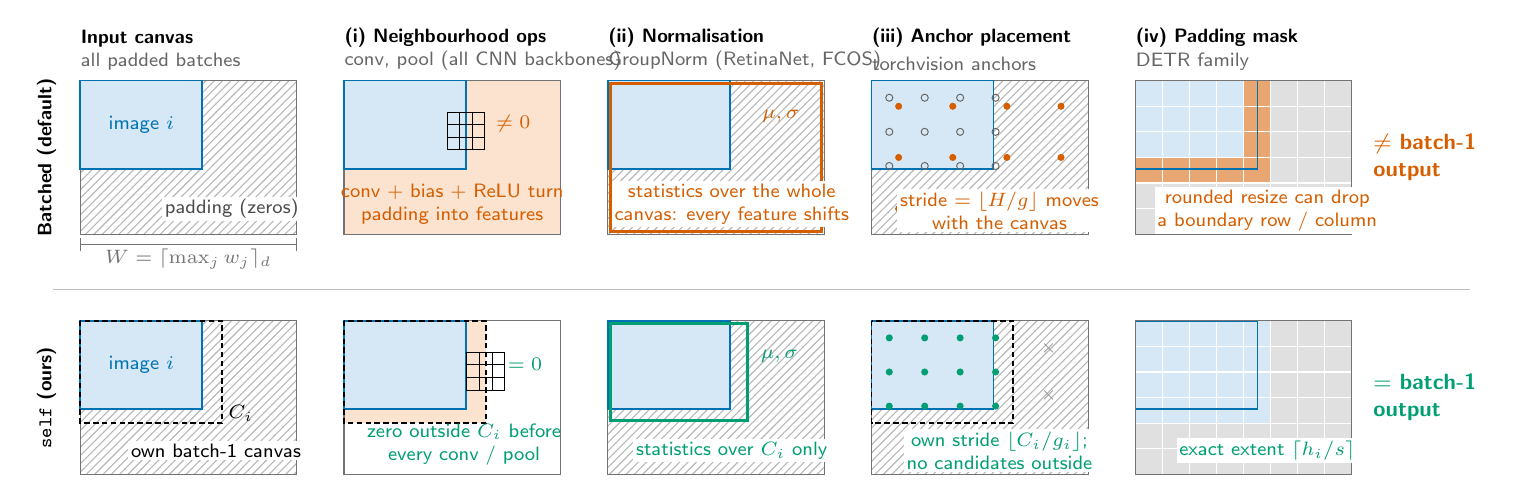
\begin{tikzpicture}[font=\fontsize{7}{8.4}\selectfont, x=1cm, y=1cm]
% geometry of one mini panel (top-left origin)
\def\W{2.75}\def\H{1.95}  % batch canvas
\def\iw{1.55}\def\ih{1.12} % image
\def\cw{1.80}\def\ch{1.30} % own batch-1 canvas C_i (rounded up)
\def\dx{3.35}              % column pitch
\def\rowA{0}\def\rowB{-3.05}
%
% ---------- helpers ----------
\newcommand{\padcanvas}[2]{% #1,#2 = top-left
  \fill[pattern=north east lines, pattern color=black!28] (#1,#2) rectangle ++(\W,-\H);
  \fill[imgfill] (#1,#2) rectangle ++(\iw,-\ih);
  \draw[black!55, line width=0.4pt] (#1,#2) rectangle ++(\W,-\H);
  \draw[oiblue, line width=0.6pt] (#1,#2) rectangle ++(\iw,-\ih);
}
\newcommand{\owncanvas}[2]{%
  \draw[black, line width=0.6pt, dash pattern=on 2pt off 1.2pt] (#1,#2) rectangle ++(\cw,-\ch);
}
%
% ---------- column headers ----------
\foreach \c/\t/\s in {0/{Input canvas}/{all padded batches},
                      1/{(i) Neighbourhood ops}/{conv, pool (all CNN backbones)},
                      2/{(ii) Normalisation}/{GroupNorm (RetinaNet, FCOS)},
                      3/{(iii) Anchor placement}/{torchvision anchors},
                      4/{(iv) Padding mask}/{DETR family}} {
  \node[anchor=south west, inner sep=0pt, font=\fontsize{7.5}{9}\selectfont\bfseries] at (\c*\dx, 0.42) {\t};
  \node[anchor=south west, inner sep=0pt, text=black!60] at (\c*\dx, 0.12) {\s};
}
% row labels
\node[rotate=90, anchor=south, font=\fontsize{7.5}{9}\selectfont\bfseries] at (-0.18, \rowA-\H/2) {Batched (default)};
\node[rotate=90, anchor=south, font=\fontsize{7.5}{9}\selectfont\bfseries] at (-0.18, \rowB-\H/2) {\texttt{self} (ours)};
%
% ======================= ROW A: default =======================
% col 0: input canvas
\padcanvas{0}{\rowA}
\node[text=oiblue] at (\iw/2, \rowA-\ih/2) {image $i$};
\node[fill=white, inner sep=1pt, text=black!70] at (\W/2+0.55, \rowA-\H+0.32) {padding (zeros)};
\draw[black!55, |-|] (0, \rowA-\H-0.13) -- node[below, inner sep=1.5pt] {$W=\lceil\max_j w_j\rceil_d$} (\W, \rowA-\H-0.13);
%
% col 1: padding becomes features
\begin{scope}[shift={(1*\dx,0)}]
  \fill[leakfill] (0,\rowA) rectangle ++(\W,-\H);
  \fill[imgfill] (0,\rowA) rectangle ++(\iw,-\ih);
  \draw[black!55, line width=0.4pt] (0,\rowA) rectangle ++(\W,-\H);
  \draw[oiblue, line width=0.6pt] (0,\rowA) rectangle ++(\iw,-\ih);
  % 3x3 kernel straddling border
  \foreach \u in {0,1,2} \foreach \v in {0,1,2}
    \draw[black, line width=0.35pt] (\iw-0.24+\u*0.16, \rowA-0.40-\v*0.16) rectangle ++(0.16,-0.16);
  \node[text=oiver] at (2.15, \rowA-0.55) {$\neq 0$};
  \node[text=oiver, align=center] at (\W/2, \rowA-\H+0.38) {conv + bias + ReLU turn\\padding into features};
\end{scope}
%
% col 2: GroupNorm over whole canvas
\begin{scope}[shift={(2*\dx,0)}]
  \padcanvas{0}{\rowA}
  \draw[oiver, line width=1.1pt] (0.03,\rowA-0.03) rectangle ++(\W-0.06,-\H+0.06);
  \node[text=oiver] at (2.2, \rowA-0.45) {$\mu,\sigma$};
  \node[fill=white, inner sep=1pt, text=oiver, align=center] at (\W/2+0.2, \rowA-\H+0.38) {statistics over the whole\\canvas: every feature shifts};
\end{scope}
%
% col 3: anchors follow the canvas
\begin{scope}[shift={(3*\dx,0)}]
  \padcanvas{0}{\rowA}
  % canvas-derived stride: 4 x 3 grid over the whole canvas
  \foreach \u in {0,...,3} \foreach \v in {0,...,2}
    \fill[oiver] ({(\u+0.5)*\W/4}, {\rowA-(\v+0.5)*\H/3}) circle (0.045);
  % own-stride positions for comparison (hollow)
  \foreach \u in {0,...,3} \foreach \v in {0,...,2}
    \draw[black!60, line width=0.35pt] ({(\u+0.5)*\cw/4}, {\rowA-(\v+0.5)*\ch/3}) circle (0.045);
  \node[fill=white, inner sep=1pt, text=oiver, align=center] at (\W/2+0.25, \rowA-\H+0.3) {stride $=\lfloor H/g\rfloor$ moves\\with the canvas};
\end{scope}
%
% col 4: rounded mask
\begin{scope}[shift={(4*\dx,0)}]
  % coarse grid 8 x 6 cells over canvas
  \pgfmathsetmacro{\gx}{\W/8}\pgfmathsetmacro{\gy}{\H/6}
  \foreach \u in {0,...,7} \foreach \v in {0,...,5} {
    \pgfmathsetmacro{\inside}{(\u<4 && \v<3) ? 1 : 0}
    \pgfmathsetmacro{\wrong}{((\u==4 && \v<4) || (\v==3 && \u<5)) ? 1 : 0}
    \ifdim\wrong pt>0.5pt
      \fill[oiver!55] (\u*\gx, \rowA-\v*\gy) rectangle ++(\gx,-\gy);
    \else\ifdim\inside pt>0.5pt
      \fill[imgfill] (\u*\gx, \rowA-\v*\gy) rectangle ++(\gx,-\gy);
    \else
      \fill[black!12] (\u*\gx, \rowA-\v*\gy) rectangle ++(\gx,-\gy);
    \fi\fi
    \draw[white, line width=0.4pt] (\u*\gx, \rowA-\v*\gy) rectangle ++(\gx,-\gy);
  }
  \draw[oiblue, line width=0.6pt] (0,\rowA) rectangle ++(\iw,-\ih);
  \draw[black!55, line width=0.4pt] (0,\rowA) rectangle ++(\W,-\H);
  \node[fill=white, inner sep=1pt, text=oiver, align=center] at (\W/2+0.3, \rowA-\H+0.3) {rounded resize can drop\\a boundary row / column};
\end{scope}
% outcome A
\node[anchor=west, text=oiver, font=\fontsize{8}{9.6}\selectfont\bfseries, align=left] at (5*\dx-0.45, \rowA-\H/2) {$\neq$ batch-1\\output};
%
% ======================= ROW B: self =======================
% col 0
\padcanvas{0}{\rowB}
\owncanvas{0}{\rowB}
\node[text=oiblue] at (\iw/2, \rowB-\ih/2) {image $i$};
\node[anchor=west, inner sep=1pt] at (\cw+0.04, \rowB-\ch+0.12) {$C_i$};
\node[fill=white, inner sep=1pt, align=center] at (\W/2+0.35, \rowB-\H+0.3) {own batch-1 canvas};
%
% col 1: zero outside C_i
\begin{scope}[shift={(1*\dx,0)}]
  \fill[white] (0,\rowB) rectangle ++(\W,-\H);
  \fill[leakfill] (0,\rowB) rectangle ++(\cw,-\ch);
  \fill[imgfill] (0,\rowB) rectangle ++(\iw,-\ih);
  \draw[black!55, line width=0.4pt] (0,\rowB) rectangle ++(\W,-\H);
  \draw[oiblue, line width=0.6pt] (0,\rowB) rectangle ++(\iw,-\ih);
  \owncanvas{0}{\rowB}
  \foreach \u in {0,1,2} \foreach \v in {0,1,2}
    \draw[black, line width=0.35pt] (\cw-0.24+\u*0.16, \rowB-0.40-\v*0.16) rectangle ++(0.16,-0.16);
  \node[text=oigreen] at (2.3, \rowB-0.55) {$=0$};
  \node[text=oigreen, align=center] at (\W/2+0.15, \rowB-\H+0.38) {zero outside $C_i$ before\\every conv / pool};
\end{scope}
%
% col 2: GN over C_i
\begin{scope}[shift={(2*\dx,0)}]
  \padcanvas{0}{\rowB}
  \draw[oigreen, line width=1.1pt] (0.03,\rowB-0.03) rectangle ++(\cw-0.06,-\ch+0.06);
  \node[text=oigreen] at (\cw+0.38, \rowB-0.45) {$\mu,\sigma$};
  \node[fill=white, inner sep=1pt, text=oigreen, align=center] at (\W/2+0.2, \rowB-\H+0.3) {statistics over $C_i$ only};
\end{scope}
%
% col 3: own anchors
\begin{scope}[shift={(3*\dx,0)}]
  \padcanvas{0}{\rowB}
  \owncanvas{0}{\rowB}
  \foreach \u in {0,...,3} \foreach \v in {0,...,2}
    \fill[oigreen] ({(\u+0.5)*\cw/4}, {\rowB-(\v+0.5)*\ch/3}) circle (0.045);
  \foreach \px/\py in {2.25/-0.35,2.25/-0.95}
    \node[text=black!45, font=\fontsize{6}{6}\selectfont] at (\px, \rowB+\py) {$\times$};
  \node[fill=white, inner sep=1pt, text=oigreen, align=center] at (\W/2+0.25, \rowB-\H+0.3) {own stride $\lfloor C_i/g_i\rfloor$;\\no candidates outside};
\end{scope}
%
% col 4: exact mask
\begin{scope}[shift={(4*\dx,0)}]
  \pgfmathsetmacro{\gx}{\W/8}\pgfmathsetmacro{\gy}{\H/6}
  \foreach \u in {0,...,7} \foreach \v in {0,...,5} {
    \pgfmathsetmacro{\inside}{(\u<5 && \v<4) ? 1 : 0}
    \ifdim\inside pt>0.5pt
      \fill[imgfill] (\u*\gx, \rowB-\v*\gy) rectangle ++(\gx,-\gy);
    \else
      \fill[black!12] (\u*\gx, \rowB-\v*\gy) rectangle ++(\gx,-\gy);
    \fi
    \draw[white, line width=0.4pt] (\u*\gx, \rowB-\v*\gy) rectangle ++(\gx,-\gy);
  }
  \draw[oiblue, line width=0.6pt] (0,\rowB) rectangle ++(\iw,-\ih);
  \draw[black!55, line width=0.4pt] (0,\rowB) rectangle ++(\W,-\H);
  \node[fill=white, inner sep=1pt, text=oigreen, align=center] at (\W/2+0.3, \rowB-\H+0.3) {exact extent $\lceil h_i/s\rceil$};
\end{scope}
% outcome B
\node[anchor=west, text=oigreen, font=\fontsize{8}{9.6}\selectfont\bfseries, align=left] at (5*\dx-0.45, \rowB-\H/2) {$=$ batch-1\\output};
%
% separator
\draw[black!25, line width=0.4pt] (-0.35, {(\rowA-\H+\rowB)/2-0.15}) -- (5*\dx+0.9, {(\rowA-\H+\rowB)/2-0.15});
\end{tikzpicture}
\end{document}
